\documentclass{beamer}
\usepackage{tikz}
% set font encoding for PDFLaTeX, XeLaTeX, or LuaTeX
\usepackage{ifxetex,ifluatex}
\if\ifxetex T\else\ifluatex T\else F\fi\fi T%
  \usepackage{fontspec}
\else
  \usepackage[T1]{fontenc}
  \usepackage[utf8]{inputenc}
  \usepackage{lmodern}
\fi

\usepackage{hyperref}

% Enable SageTeX to run SageMath code right inside this LaTeX file.
% http://doc.sagemath.org/html/en/tutorial/sagetex.html
% \usepackage{sagetex}

% Enable PythonTeX to run Python – https://ctan.org/pkg/pythontex
% \usepackage{pythontex}

\begin{document}


\begin{frame}{Three cores}
\begin{center}
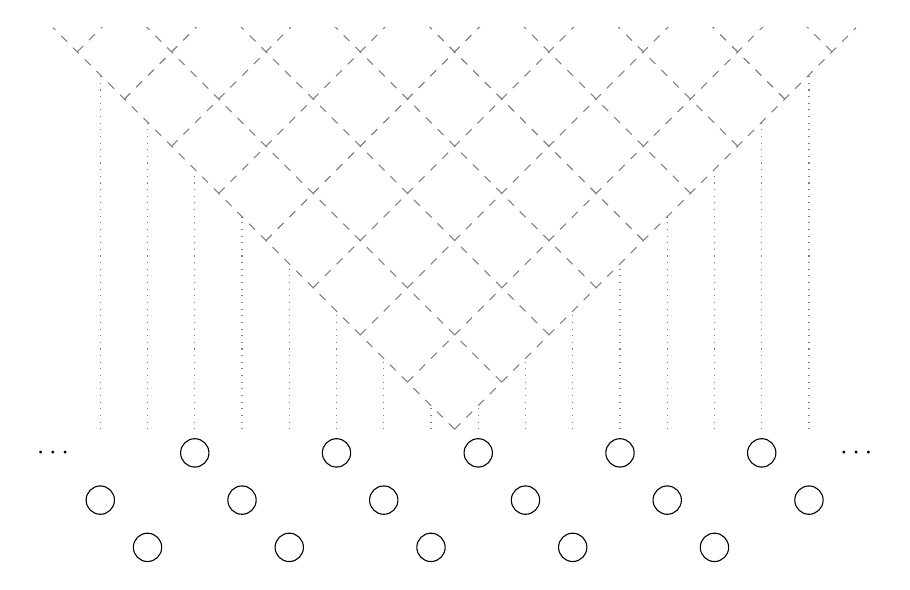
\begin{tikzpicture}
\begin{scope}[gray, very thin, scale=.6]
   \clip (-8.5, 8.5) rectangle (8.5, -1);
   \draw[rotate=45, scale=1.412, thin, gray, dashed] (0,0) grid (10,10);
\end{scope}
\begin{scope}[scale=.6, yshift=-.5cm]
   \draw (-8.5,0) node{$\cdots$};
     \draw (-7.5,-1) circle (.3);

 \draw (-6.5,-2) circle (.3);
   \draw (-5.5,0) circle (.3);

 \draw (-4.5,-1) circle (.3);
   \draw (-3.5,-2) circle (.3);
   \draw (-2.5,0) circle (.3);
   \draw (-1.5,-1) circle (.3);
   \draw (-.5,-2) circle (.3);
   \draw (.5,0) circle (.3);
   \draw (1.5,-1) circle (.3);
   \draw (2.5,-2) circle (.3);
   \draw (3.5,0) circle (.3);
   \draw (4.5,-1) circle (.3);
   \draw (5.5,-2) circle (.3);
   \draw (6.5,0) circle (.3);
    \draw (7.5,-1) circle (.3);

\draw (8.5,0) node{$\cdots$};
  \end{scope}

\begin{scope}[scale=.6]
\foreach \x in {.5, 1.5,...,6.5,7.5} {
\draw[thin, dotted, gray] (\x,0) -- (\x, \x);
\draw[thin, dotted, gray] (-\x,0) -- (-\x, \x); };

\end{scope}

\end{tikzpicture}


\end{center}

\end{frame}







\end{document}
